\begin{exercice*}
    Pour chaque situation, dire si la figure $\mathcal{F}_2$ est l'image de la figure $\mathcal{F}_1$ par une homothétie.

    Préciser son centre et son rapport le cas échéant.
    
    \begin{enumerate}
        \item \phantom{rrr}
        
        \begin{tikzpicture}[scale=0.6]
            \draw[help lines, color=black!30] (0,0) grid (12,4);
            % Points 
            \coordinate (O) at (1,0);
            \coordinate (A) at (2.5,0);
            \coordinate (B) at (4.5,0);
            \coordinate (C) at (2.5,1);
            \tkzDefBarycentricPoint(A=1,B=1,C=1)
            \tkzGetPoint{F1}            
            \tkzDefPointBy[homothety=center O ratio 3](A); \tkzGetPoint{A'};
            \tkzDefPointBy[homothety=center O ratio 3](B); \tkzGetPoint{B'};
            \tkzDefPointBy[homothety=center O ratio 3](C); \tkzGetPoint{C'};            
            \tkzDefBarycentricPoint(A'=1,B'=1,C'=1)
            \tkzGetPoint{F2}            
            % Tracés
            \tkzDrawPoints[shape=cross out,size=3pt](O);
            \draw[fill=gray, fill opacity=0.2] (A)--(B)--(C)--cycle;
            \draw[fill=gray, fill opacity=0.2] (A')--(B')--(C')--cycle;
            \tkzLabelPoint[above,shift={(0,-0.3)}](F1){$\mathcal{F}_1$};
            \tkzLabelPoint[above,shift={(0,-0.3)}](F2){$\mathcal{F}_2$};
            \tkzLabelPoints[above](O);
        \end{tikzpicture}
        \item \phantom{rrr}
        
        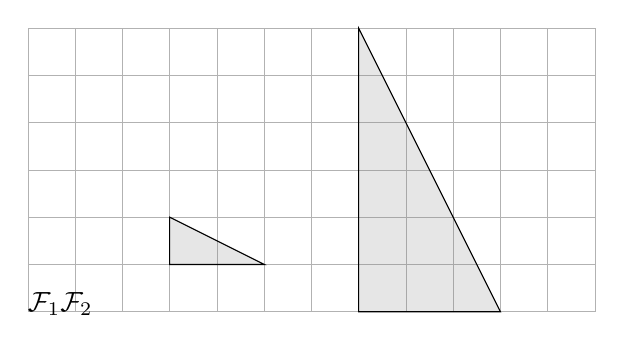
\begin{tikzpicture}[scale=0.6]
            \draw[help lines, color=black!30] (0,0) grid (12,6);
            % Points 
            \coordinate (O) at (1,0);
            \coordinate (A) at (3,1);
            \coordinate (B) at (5,1);
            \coordinate (C) at (3,2);
            \tkzDefBarycentricPoint(A=1,B=1,C=1)
            \tkzGetPoint{F1}            
            \coordinate (A') at (7,0);
            \coordinate (B') at (7,6);
            \coordinate (C') at (10,0);
            \tkzDefBarycentricPoint(A'=1,B'=1,C'=1)
            \tkzGetPoint{F2}            
            % Tracés
            \tkzDrawPoints[shape=cross out,size=3pt](O);
            \draw[fill=gray, fill opacity=0.2] (A)--(B)--(C)--cycle;
            \draw[fill=gray, fill opacity=0.2] (A')--(B')--(C')--cycle;
            \tkzLabelPoint[above,shift={(0,-0.3)}](F1){$\mathcal{F}_1$};
            \tkzLabelPoint[above,shift={(0,0)}](F2){$\mathcal{F}_2$};
            \tkzLabelPoints[above](O);
        \end{tikzpicture}
        \item \phantom{rrr}
        
        \begin{tikzpicture}[scale=0.6]
            \draw[help lines, color=black!30] (0,0) grid (12,6);
           % Points 
           \coordinate (O) at (1,0);
           \coordinate (A) at (2,1);
           \coordinate (B) at (4,1);
           \coordinate (C) at (2,2);
           \tkzDefBarycentricPoint(A=1,B=1,C=1)
           \tkzGetPoint{F2}            
           \tkzDefPointBy[homothety=center O ratio 3](A); \tkzGetPoint{A'};
           \tkzDefPointBy[homothety=center O ratio 3](B); \tkzGetPoint{B'};
           \tkzDefPointBy[homothety=center O ratio 3](C); \tkzGetPoint{C'};            
           \tkzDefBarycentricPoint(A'=1,B'=1,C'=1)
           \tkzGetPoint{F1}            
           % Tracés
           \tkzDrawPoints[shape=cross out,size=3pt](O);
           \draw[fill=gray, fill opacity=0.2] (A)--(B)--(C)--cycle;
           \draw[fill=gray, fill opacity=0.2] (A')--(B')--(C')--cycle;
           \tkzLabelPoint[above,shift={(0,-0.3)}](F1){$\mathcal{F}_1$};
           \tkzLabelPoint[above,shift={(0,-0.3)}](F2){$\mathcal{F}_2$};
           \tkzLabelPoints[above](O);
        \end{tikzpicture}
    \end{enumerate}
\end{exercice*}
\begin{corrige}
    %\setcounter{partie}{0} % Pour s'assurer que le compteur de \partie est à zéro dans les corrigés
    % \phantom{rrr}
    Pour chaque situation, dire si la figure $\mathcal{F}_2$ est l'image de la figure $\mathcal{F}_1$ par une homothétie.

    Préciser son centre et son rapport le cas échéant.
    
    \begin{enumerate}
        \item {\color{red} $\mathcal{F}_2$ est l'image de $\mathcal{F}_1$ par l'homothétie de centre $O$ et de rapport $3$.}
        
        \begin{tikzpicture}[scale=0.6]
            \draw[help lines, color=black!30] (0,0) grid (12,4);
            % Points 
            \coordinate (O) at (1,0);
            \coordinate (A) at (2.5,0);
            \coordinate (B) at (4.5,0);
            \coordinate (C) at (2.5,1);
            \tkzDefBarycentricPoint(A=1,B=1,C=1)
            \tkzGetPoint{F1}            
            \tkzDefPointBy[homothety=center O ratio 3](A); \tkzGetPoint{A'};
            \tkzDefPointBy[homothety=center O ratio 3](B); \tkzGetPoint{B'};
            \tkzDefPointBy[homothety=center O ratio 3](C); \tkzGetPoint{C'};            
            \tkzDefBarycentricPoint(A'=1,B'=1,C'=1)
            \tkzGetPoint{F2}            
            % Tracés
            \tkzDrawPoints[shape=cross out,size=3pt](O);
            \draw[fill=gray, fill opacity=0.2] (A)--(B)--(C)--cycle;
            \draw[fill=gray, fill opacity=0.2] (A')--(B')--(C')--cycle;
            \tkzLabelPoint[above,shift={(0,-0.3)}](F1){$\mathcal{F}_1$};
            \tkzLabelPoint[above,shift={(0,-0.3)}](F2){$\mathcal{F}_2$};
            \tkzLabelPoints[above](O);
        \end{tikzpicture}
        \item {\color{red} L'orientation n'est pas la même, $\mathcal{F}_2$ n'est donc pas l'image de $\mathcal{F}_1$ par une homothétie.}
        
        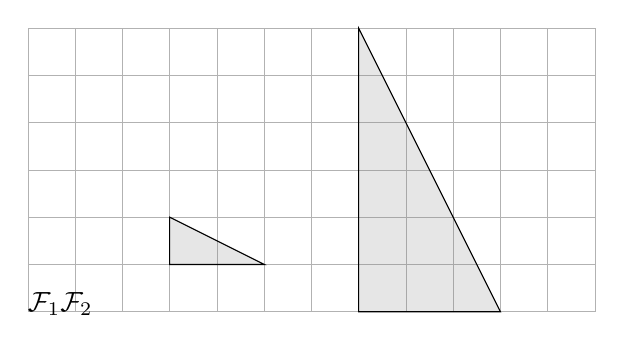
\begin{tikzpicture}[scale=0.6]
            \draw[help lines, color=black!30] (0,0) grid (12,6);
            % Points 
            \coordinate (O) at (1,0);
            \coordinate (A) at (3,1);
            \coordinate (B) at (5,1);
            \coordinate (C) at (3,2);
            \tkzDefBarycentricPoint(A=1,B=1,C=1)
            \tkzGetPoint{F1}            
            \coordinate (A') at (7,0);
            \coordinate (B') at (7,6);
            \coordinate (C') at (10,0);
            \tkzDefBarycentricPoint(A'=1,B'=1,C'=1)
            \tkzGetPoint{F2}            
            % Tracés
            \tkzDrawPoints[shape=cross out,size=3pt](O);
            \draw[fill=gray, fill opacity=0.2] (A)--(B)--(C)--cycle;
            \draw[fill=gray, fill opacity=0.2] (A')--(B')--(C')--cycle;
            \tkzLabelPoint[above,shift={(0,-0.3)}](F1){$\mathcal{F}_1$};
            \tkzLabelPoint[above,shift={(0,0)}](F2){$\mathcal{F}_2$};
            \tkzLabelPoints[above](O);
        \end{tikzpicture}
        \item {\color{red} $\mathcal{F}_2$ est l'image de $\mathcal{F}_1$ par l'homothétie de centre $O$ et de rapport $\dfrac{1}{3}$.}
        
        \begin{tikzpicture}[scale=0.6]
            \draw[help lines, color=black!30] (0,0) grid (12,6);
           % Points 
           \coordinate (O) at (1,0);
           \coordinate (A) at (2,1);
           \coordinate (B) at (4,1);
           \coordinate (C) at (2,2);
           \tkzDefBarycentricPoint(A=1,B=1,C=1)
           \tkzGetPoint{F2}            
           \tkzDefPointBy[homothety=center O ratio 3](A); \tkzGetPoint{A'};
           \tkzDefPointBy[homothety=center O ratio 3](B); \tkzGetPoint{B'};
           \tkzDefPointBy[homothety=center O ratio 3](C); \tkzGetPoint{C'};            
           \tkzDefBarycentricPoint(A'=1,B'=1,C'=1)
           \tkzGetPoint{F1}            
           % Tracés
           \tkzDrawPoints[shape=cross out,size=3pt](O);
           \draw[fill=gray, fill opacity=0.2] (A)--(B)--(C)--cycle;
           \draw[fill=gray, fill opacity=0.2] (A')--(B')--(C')--cycle;
           \tkzLabelPoint[above,shift={(0,-0.3)}](F1){$\mathcal{F}_1$};
           \tkzLabelPoint[above,shift={(0,-0.3)}](F2){$\mathcal{F}_2$};
           \tkzLabelPoints[above](O);
        \end{tikzpicture}
    \end{enumerate}
\end{corrige}

